\documentclass[letterpaper,12pt]{article}

\usepackage[utf8x]{inputenc}
\usepackage[T1]{fontenc}
\usepackage{times}
\usepackage[colorlinks=true,linkcolor=black,citecolor=black,urlcolor=blue]{hyperref}
\usepackage{geometry}
\geometry{top=0.9in,bottom=0.9in,left=0.9in,right=0.9in}
\pagestyle{empty}

\usepackage{titlesec}
\titleformat{\section}
{\bfseries\uppercase}{\thesection.}{1em}{}
\titleformat{\subsection}
{\bfseries}{\thesection.\thesubsection.}{1em}{}
\renewcommand{\labelitemi}{\textendash}
\renewcommand{\labelitemii}{\textendash}

\usepackage{graphicx} % used to insert the figure
\usepackage{multirow} % used for the table
%\usepackage[font=it]{caption}
\usepackage{cite}
\usepackage{breakurl}
\usepackage{indentfirst}
\usepackage{amsmath, amssymb, amsfonts, bm}
\usepackage{txfonts}
\usepackage{enumitem}
\usepackage{xcolor}
\usepackage{enumitem}
\usepackage{caption}
\usepackage{subcaption}

\hyphenpenalty=10000
\setlength{\emergencystretch}{3em}

\columnsep 1cm
\setlength{\parindent}{0.5cm}

\titlespacing*{\subsection}{0pt}{1.5em}{0.2em}

\renewcommand\eqref[1]{Equation~\ref{#1}}
\renewcommand{\thesection}{\arabic{section}}
\renewcommand{\thesubsection}{\arabic{subsection}}
\renewcommand{\arraystretch}{1.25}
\renewcommand{\refname}{REFERENCES} 
\setlength{\footnotesep}{12pt} 
\newlength{\bibitemsep}\setlength{\bibitemsep}{.2\baselineskip plus .05\baselineskip minus .05\baselineskip}
\newlength{\bibparskip}\setlength{\bibparskip}{0pt}
\let\oldthebibliography\thebibliography
\renewcommand\thebibliography[1]{%
  \oldthebibliography{#1}%
  \setlength{\parskip}{\bibitemsep}%
  \setlength{\itemsep}{\bibparskip}%
}
 
\begin{document}

\begin{center}
    
\includegraphics[width=2.65in]{fig/logo_NC23.jpg}
\end{center}
\vskip.5cm

\begin{flushleft}
\fontsize{16}{20}\selectfont\bfseries
\color{black}Sound power characterization of Corsi-Rosenthal boxes using DIY comparison method
\end{flushleft}
\vskip1cm

\renewcommand\baselinestretch{1}
\begin{flushleft}

John Arthur Case\footnote{jac7175@psu.edu}, Carter Paprocki\footnote{cap6296@psu.edu}, Hannah Kurdila\footnote{hrk5147@psu.edu}, Trent Furlong\footnote{tsf44@psu.edu}, Eric Rokni\footnote{ezr144@psu.edu}, Yu-Tong Wang\footnote{ybw5392@psu.edu}, Jiaxin Zhong\footnote{Jiaxin.Zhong@psu.edu}, Jun Ji\footnote{jbj5431@psu.edu}, Daniel Russell\footnote{dar119@psu.edu}, Andrew Barnard\footnote{barnard@psu.edu}\\
The Pennsylvania State University Graduate Program in Acoustics\\
201 Applied Science Building
University Park, PA 16802, United States\\

\end{flushleft}


\textbf{\centerline{ABSTRACT}}\\
\textit{Corsi-Rosenthal (CR) boxes efficiently and cost-effectively clean the air in an environment; however, the constant broadband noise they produce is a concern. Measuring sound power levels of CR boxes would provide a metric for noise comparisons, but traditional sound power level measurements are not readily adaptable for the average consumer. Measuring the sound power level in a free field over a reflecting plane is an accurate method but is complicated and expensive involving multiple microphones in an anechoic chamber (ANSI S12.54-1999). The Comparison Method is a simpler procedure that can be performed directly in the environment of interest but requires an expensive calibrated source (ANSI S12.57-2011). To allow for simple and inexpensive sound power measurements of CR boxes, we used ANSI S12.54-1999 to measure the sound power of a \$30 hand vacuum (Black+Decker HNVC115JB06) to explore its potential as a DIY calibrated source for the Comparison Method. The reproducibility and uncertainty of this DIY method will be discussed. The DIY method has the potential to enable noise comparison of air cleaners or other devices for the average consumer.}

\section{INTRODUCTION}
\noindent

Indoor air quality became a focus during the COVID-19 pandemic \cite{mousavi2020covid, zhao2020air}.
Corsi-Rosenthal Boxes are do-it-yourself (DIY) filtration systems that give the average consumer the ability to improve indoor air quality and reduce exposure to COVID-19 in smaller settings\cite{dodson2022does, dal2022characterizing,rosenthal2022variation}. They are inexpensive to build, portable, and only require a standard electrical outlet to power. While Corsi-Rosenthal boxes offer flexible filtration benefits, the noise they produce is a potential problem for consumers. They can cause annoyance, listening fatigue, and a reduction in speech intelligibility \cite{houtgast1980predicting}. It is also desired to compare of-the-shelf air purifiers to DIY options. As such, it is beneficial for consumers to make their own sound characterization measurements \textit{in situ}.

Sound power is a source quantity that allows for accurate comparison of two sound sources. Knowing the sound power of a source allows for the prediction of the sound pressure level in a room, assuming the room's acoustic properties are known. This relation is given be the following equation:
\begin{equation}
    L_p = L_w + 10\log_{10} \left(\frac{D}{4\pi r^2} + \frac{4}{R} \right)-A 
\end{equation}
where $L_p$ is sound pressure level, $L_w$ is sound power level, $D$ is source directivity, $ r$ is the distance from the source to the receiver, $R$ is the room constant and $A$ is an accumulative excess attenuation.   

The comparison method (see ANSI S12.57-2011) provides a way to evaluate the sound power of a sound source \textit{in situ} but relies on an expensive calibrated sound power source \cite{S12.57-2011}. These calibrated sources provide constant broadband sound power and can remain consistent for decades.  For consumer applications, it would be beneficial to have an inexpensive sound source that could be used in place of a traditional calibrated source while still providing reliable broadband sound energy. The comparison method also allows for the use of an uncalibrated microphone (including cellphone-based microphones) to make measurements. The goal of this work is to verify the effectiveness of using an inexpensive hand vacuum as a calibrated source for the comparison method. The sound power of multiple hand vacuums were measured according to ANSI S12.54-2011 and the variability of these results were explored  \cite{S12.54-2011}. The hand vacuums were then used with the DIY comparison method to measure sound power levels of the Corsi-Rosental box. 
 
\section{METHODS}
\noindent

%The scope of this experimental work consists of two main steps: First, measure the ground truth sound power level of a consumer good using ANSI S12.54-1999 to create a calibration curve. Second, test the new calibrated source using the comparison method found in ANSI S12.57-2011. This new calibrated source would then be able to be purchased at most places around the world and accurately calculate sound power of the Corsi-Rosenthal boxes.
 
 Several inexpensive (<\$100) objects including an angle grinder, electric air pump, small vacuum cleaner, and white noise generator were chosen as candidates to be used as a ``calibrated'' reference sound power source. The sound power of these objects were measured in a hemi-anechoic chamber over a reflective floor according to ANSI S12.54-2011. For this, four random incidence microphones were placed in an arc around the object in accordance with Table B.1 in ANSI S12.54-2011 at a radius of 1m. Data was acquired using a four-channel Crystal Instruments Spider 20-HE for a duration of 20 seconds at a sampling rate of 44.1 kHz. Sound pressure was recorded at each microphone at $60^{\circ}$ increments around the source origin. Sound power levels were reported in one-third octave bands and compared against the calibrated source, as shown in Figure \ref{fig:SourceComparison}. Despite showing the most favorable broadband sound power, the angle grinder was not chosen due to its higher cost, requirement to be plugged in to mains voltage, and potential danger associated with operation. Thus, the handheld vacuum cleaner was chosen as a safer, more affordable option that still provided a sufficient broadband sound power. The sound power levels of six hand vacuums of similar makes and models (4x Black \& Decker HNVC115J, 2x Dirt Devil BB30008) were then measured in the same manner to ensure repeatable sound profiles across the same model vacuums. Due to the small sample size and large variability in power across frequencies for the Dirt Devil vacuums, the Black \& Decker vacuums were chosen as the DIY reference source for subsequent measurements.

\begin{figure}[h!]
    \centering
    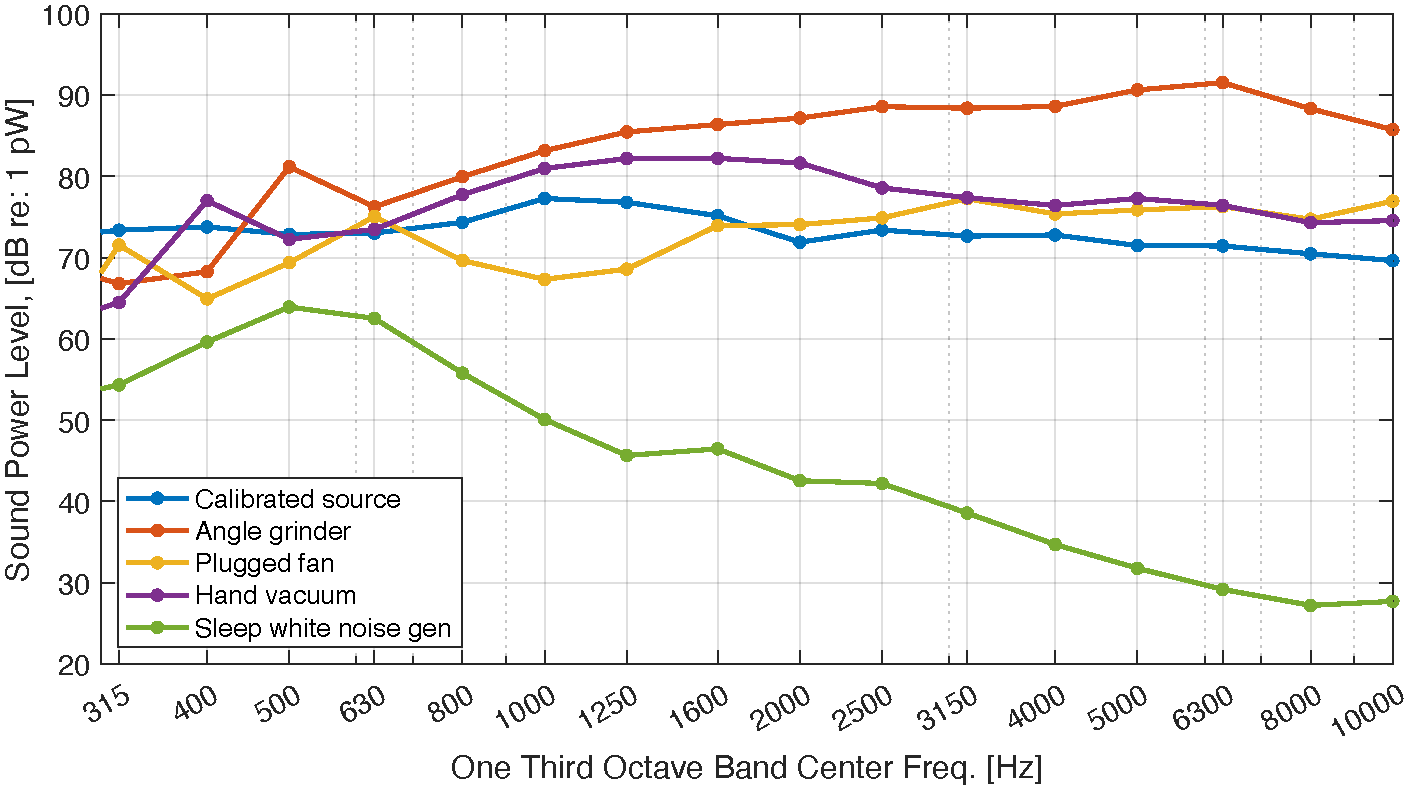
\includegraphics[width=0.9\textwidth]{manuscript/fig/SourceComparison}
    \caption{Sound power level measurements of several common consumer goods and a calibrated sound power source.}
    \label{fig:SourceComparison}
\end{figure}

The sound power of the Corsi-Rosenthal box was measured in a standard office setting using the comparison method with hand vacuums as the reference sound power source. Single channel sound pressure levels of the Corsi-Rosenthal box, $\overline{L_{p}}$, were recorded with a B\&K 2250 Sound Level Meter (SLM), shown in Figure \ref{fig:ComparisonTest}. A surface average of the sound pressure level was measured by walking around the source for 60 seconds. This procedure was performed for each of the three fan settings. Next, the hand vacuums were measured with the same technique to get the the reference source sound pressure level, $\overline{L_{p_r}}$. The sound power of the Corsi-Rosenthal box ($L_w$) could then be calculated with $L_{w} = L_{w_r} + \overline{L_{p}} - \overline{L_{p_r}}\label{eqn:Lw}$, where $L_{w_r}$ is the sound power level of the hand vacuum.

A ``ground-truth'' sound power level of the Corsi-Rosenthal box was measured using the hemi-anechoic method, described earlier and shown in Figure \ref{fig:CorsiHemi}. A microphone radius of 2m was used to ensure far-field measurements. The calculated sound power using the comparison method was then validated against this measurement.

\begin{figure}[h!]
\centering
\begin{minipage}{.48\textwidth}
  \centering
  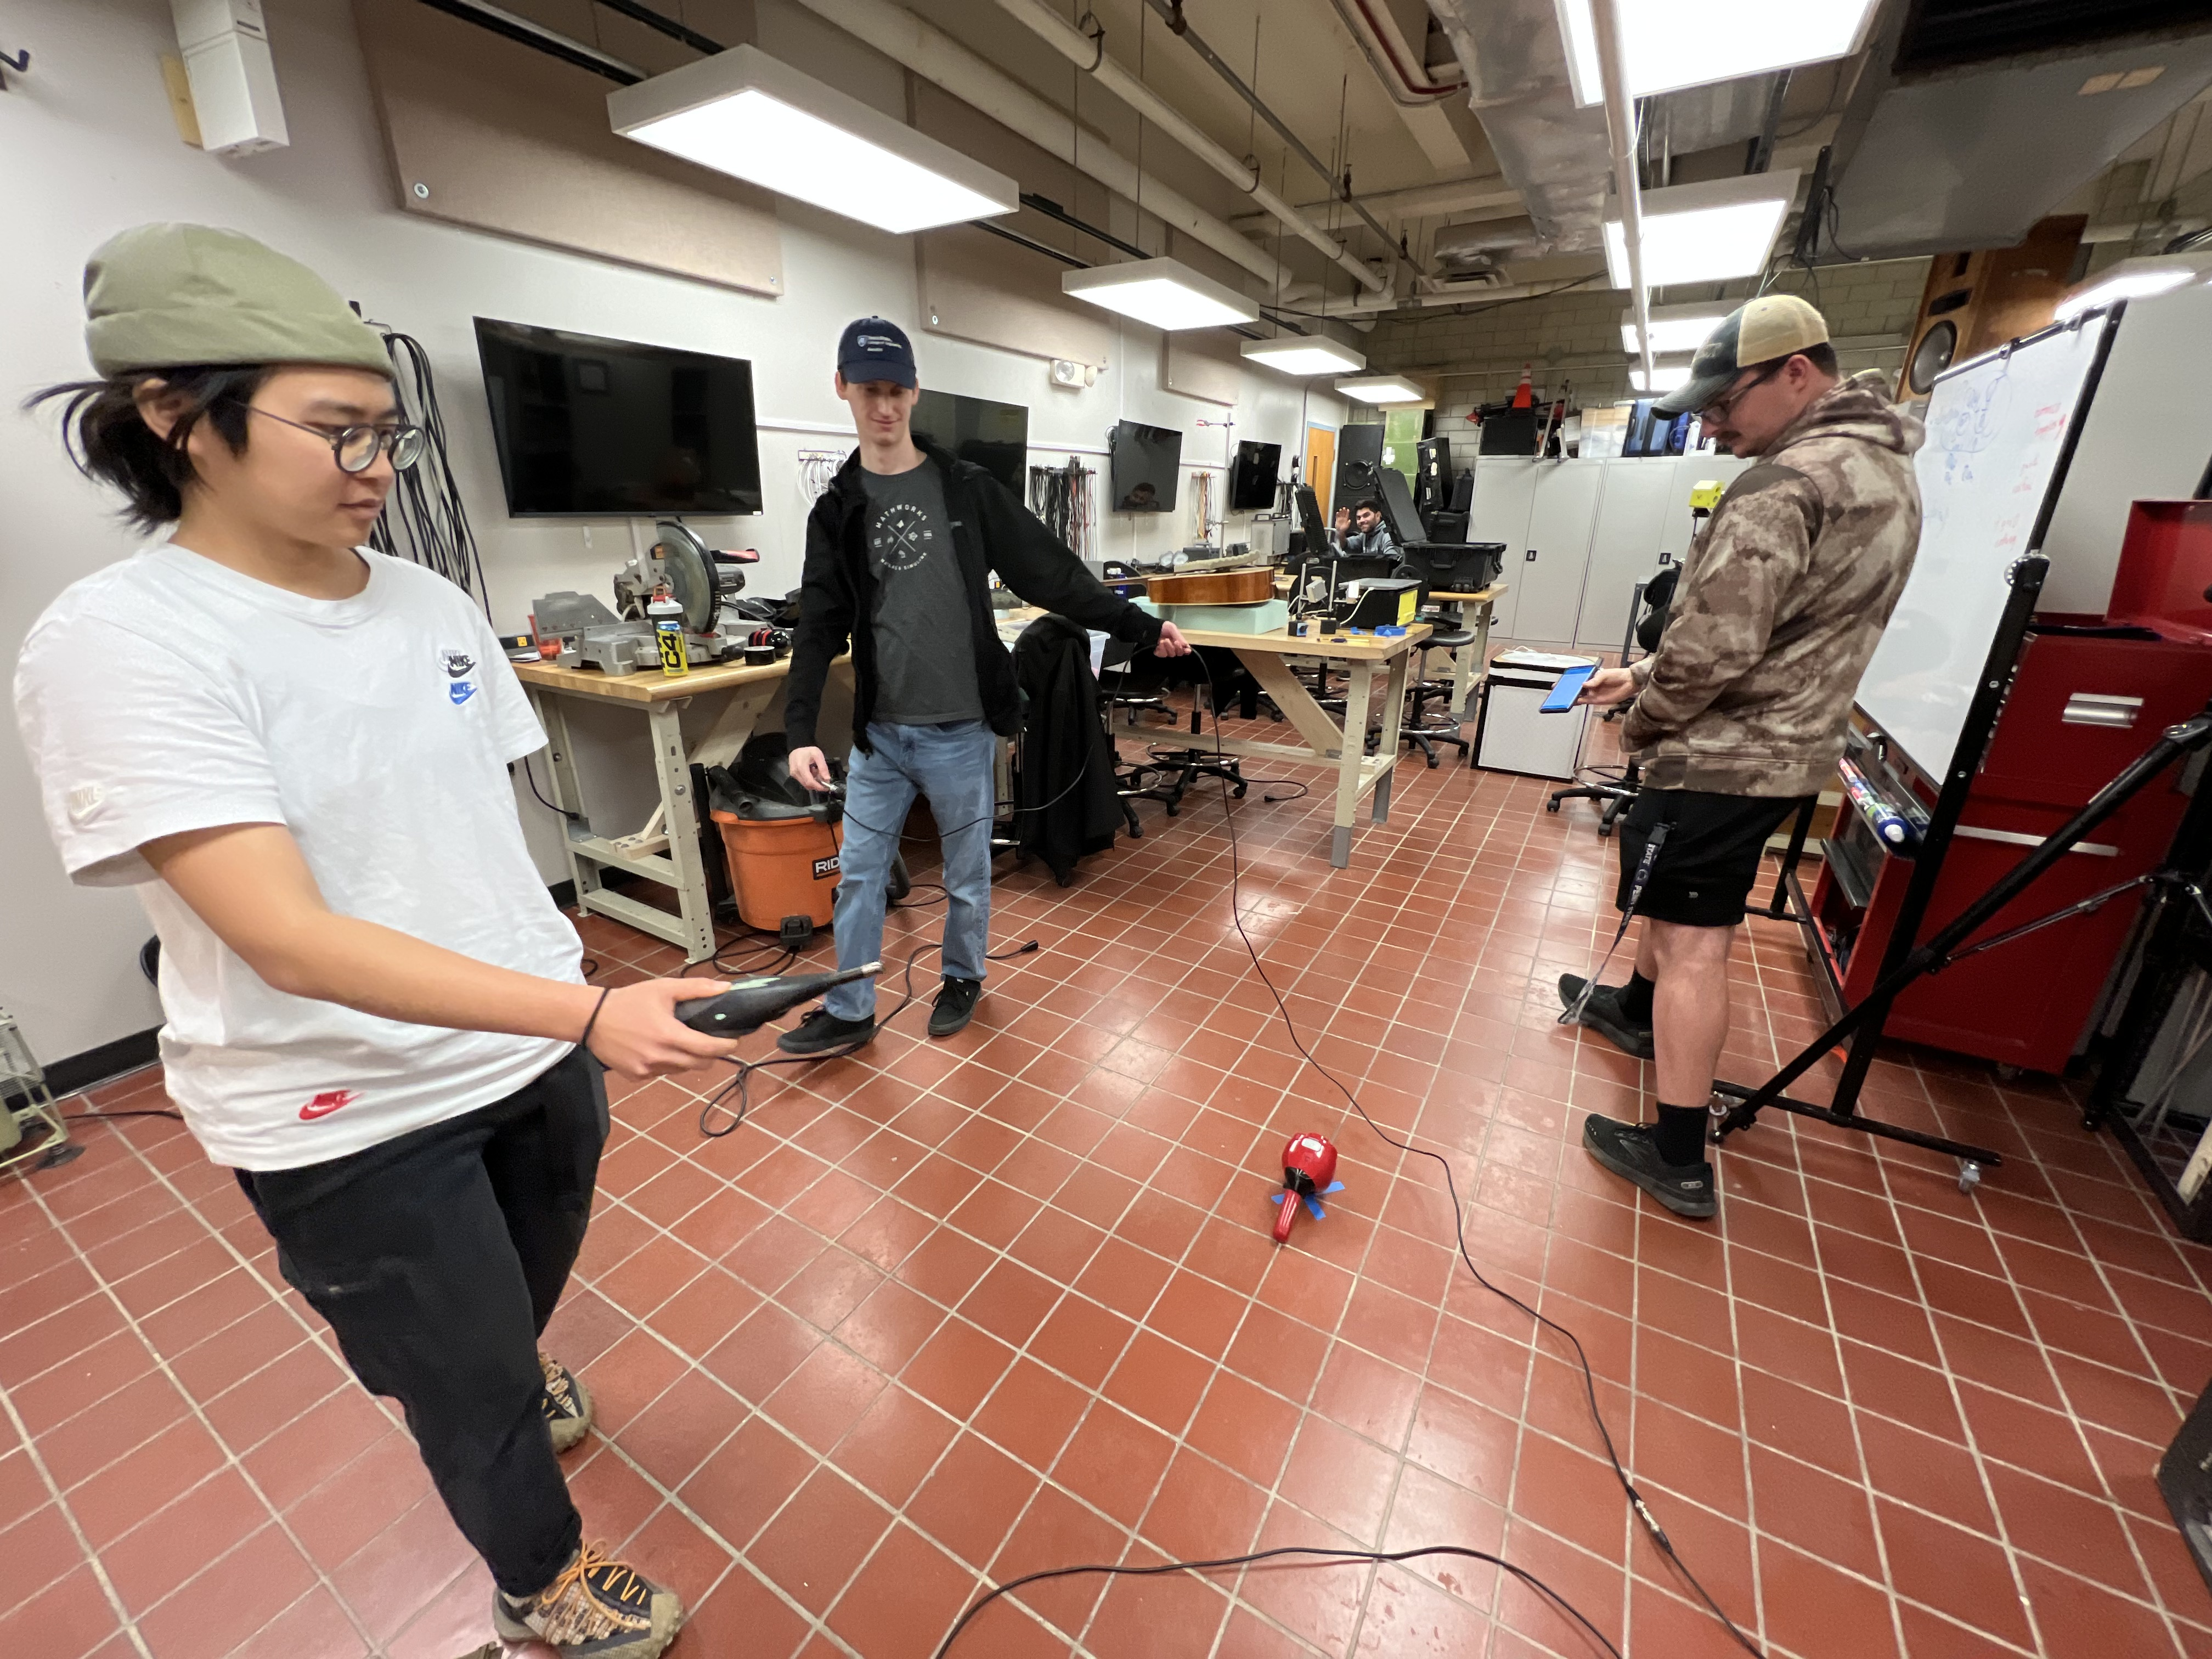
\includegraphics[width=0.95\linewidth]{manuscript/fig/ComparisonTest}
  \captionof{figure}{Measuring the time and spatially averaged sound pressure levels for the hand vacuum and Corsi-Rosenthal box in the lab.}
  \label{fig:ComparisonTest}
\end{minipage}%
\hfill
\begin{minipage}{.48\textwidth}
  \centering
  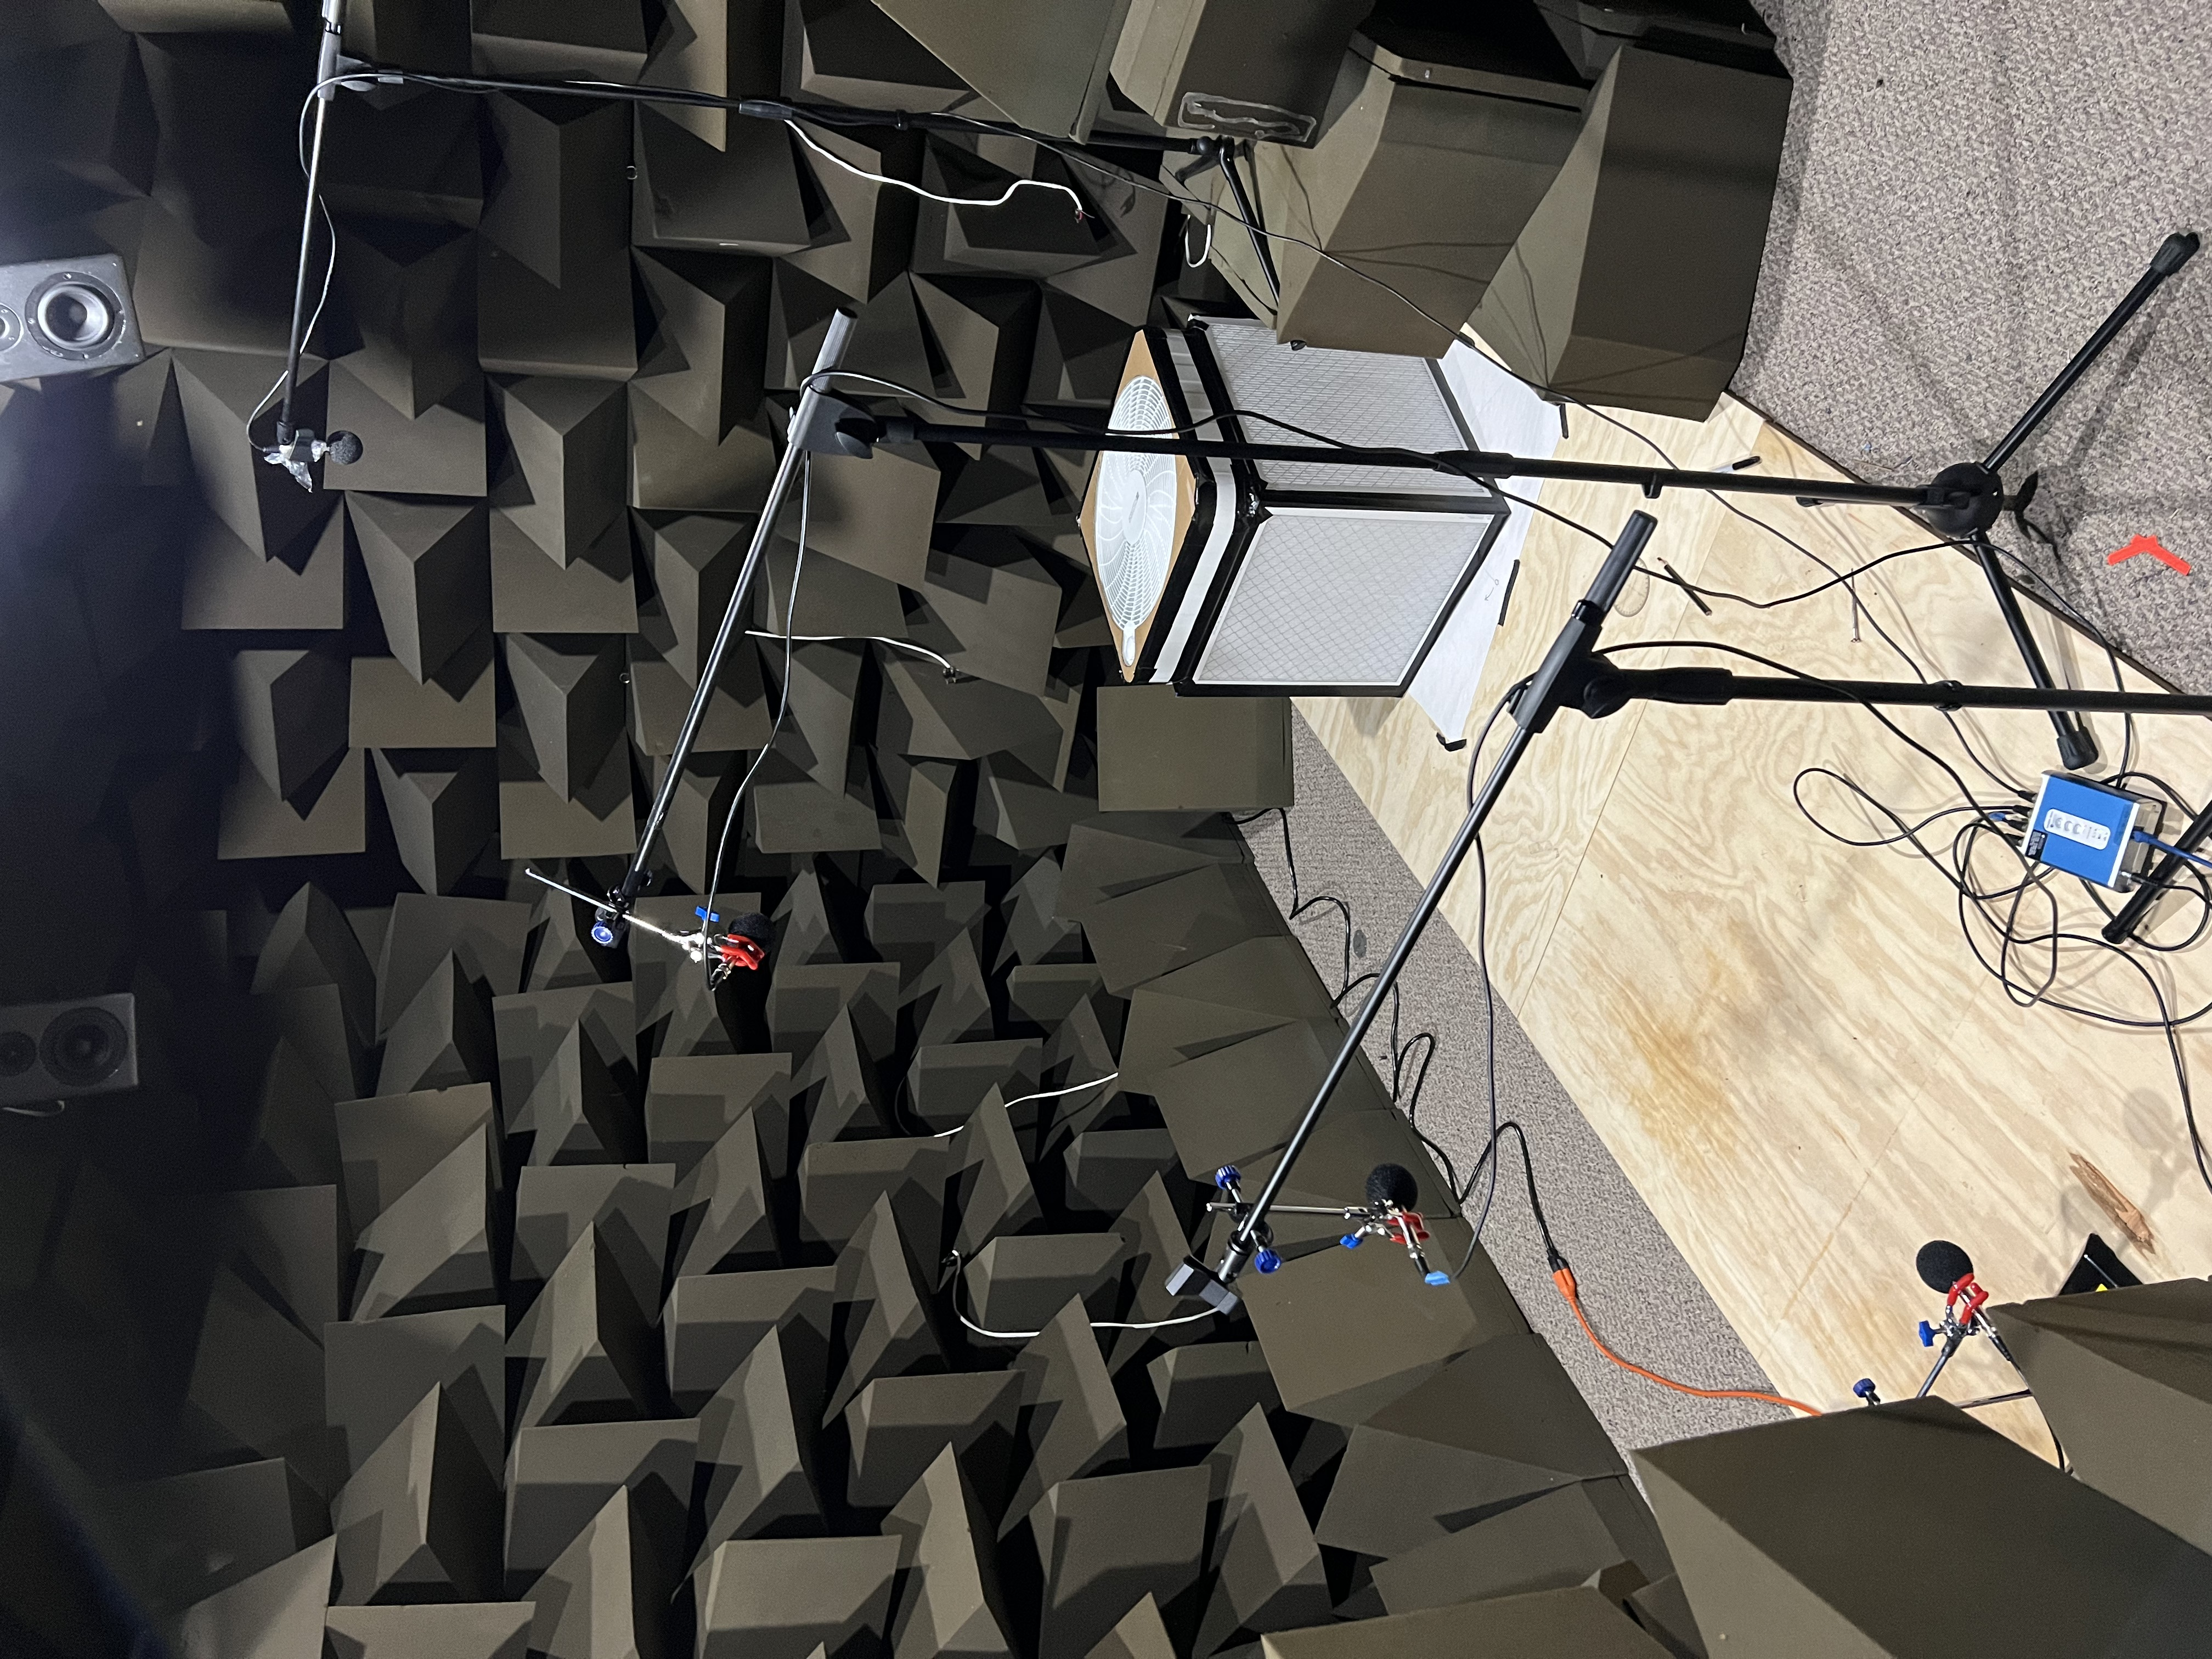
\includegraphics[width=0.95\linewidth,angle=270]{manuscript/fig/CorsiHemi}
  \captionof{figure}{Anechoic chamber testing of ANSI S12.54-2011 to calculate the sound power of a Corsi-Rosenthal box using a 2 meter microphone radius.}
  \label{fig:CorsiHemi}
\end{minipage}
\end{figure}

\pagebreak
\section{Results}
The averaged sound power levels of the six tested hand vacuums are given in Figure \ref{fig:HemiVac}. Within each vacuum type, standard deviations were less than 3 dB across most frequency bands. The Black \& Decker vacuums provided relatively constant broadband noise above 55 dB in the one-third octave bands above 630 Hz. The Dirt Devil vacuums showed large variations across frequency bands.
\begin{figure}[h!]
    \centering
    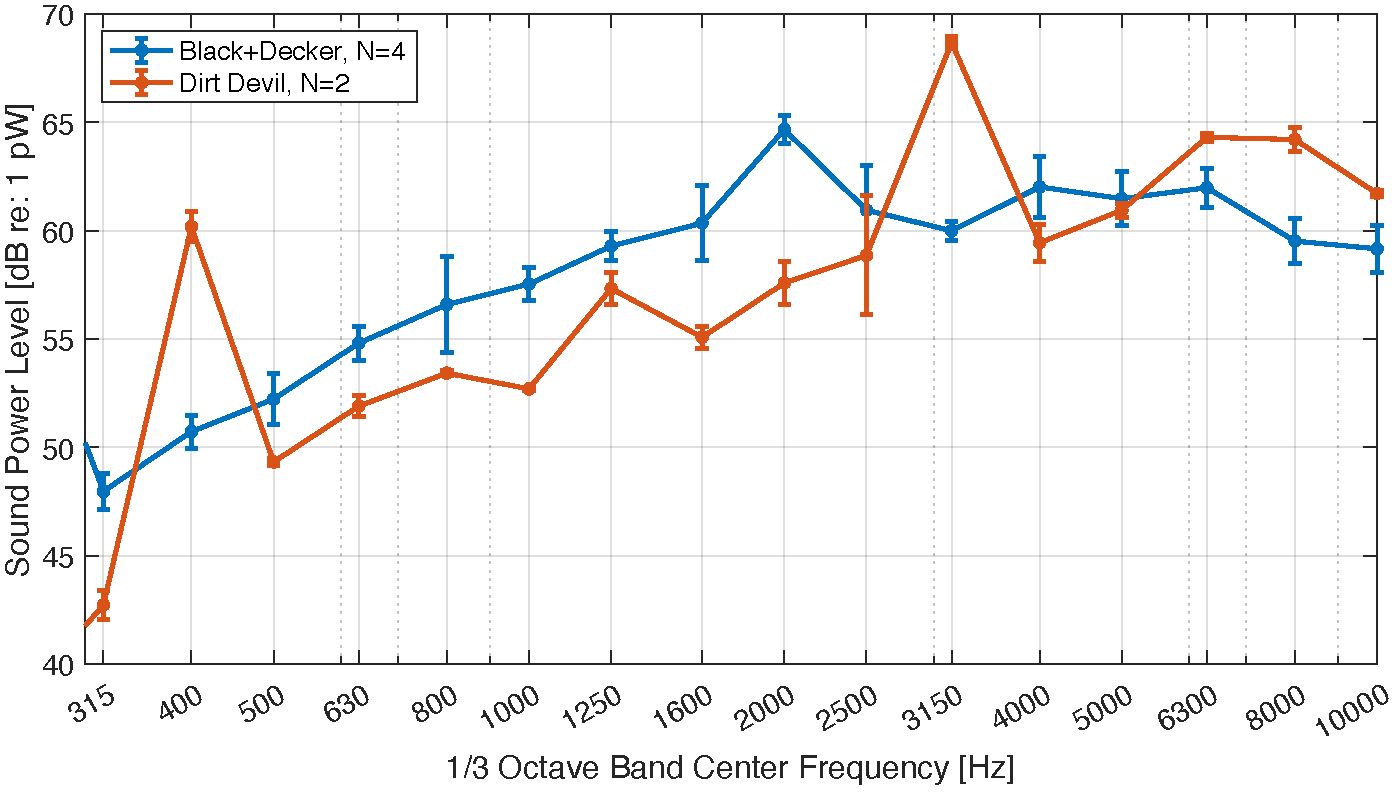
\includegraphics[width=0.9\textwidth]{manuscript/fig/HemiVac.pdf}
    \caption{Average sound power level of Black \& Decker (blue) and Dirt Devil (orange) vacuums, as measured using the hemi-anechoic method.}
    \label{fig:HemiVac}
\end{figure}
The ``ground-truth'' sound power of the Corsi-Rosenthal for all three fan settings are presented in Figure \ref{fig:GroundTruth}. All three fan settings produced consistent sound profiles across all frequencies. As fan setting 3 had the highest overall sound power level, all subsequent analyses referenced this setting.

The sound power levels of the Corsi-Rosenthal box as measured using the hemi-anechoic method, and comparison method using a Type 1 SLM are provided in Figure \ref{fig:comparisonfan3} for the highest fan speed. The DIY comparison method shows a promising similarity to the base results found using the hemi-anechoic method. Over the frequency range of interest, the DIY method gave results within 1.7 dB of the ``ground-truth'' at a 95\% confidence interval.   
\begin{figure}[h!]
    \centering
    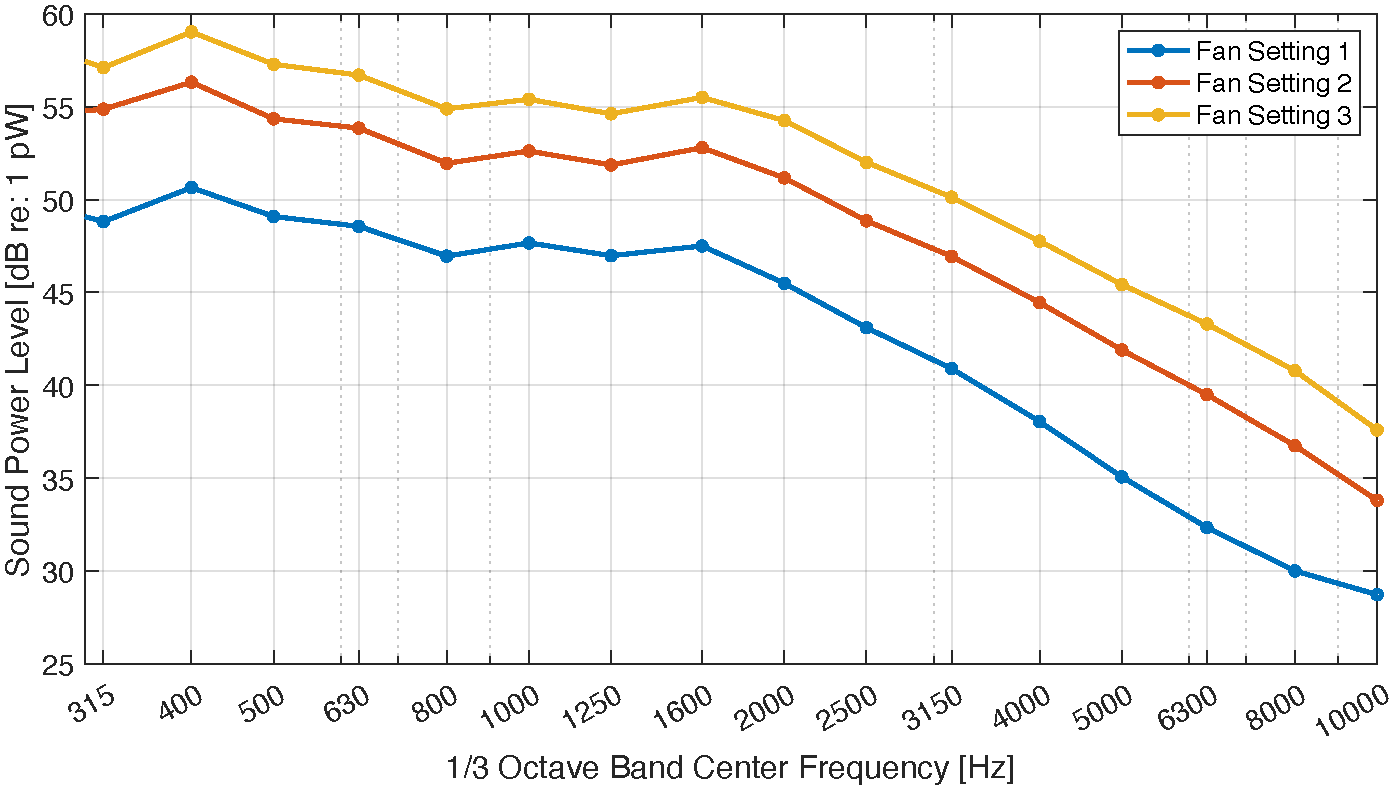
\includegraphics[width=0.9\textwidth]{manuscript/fig/CorsiLwHemiAnech.pdf}
    \caption{Sound power level of the Corsi-Rosenthal Box as measured by the hemi-anechoic method for each fan setting.}
    \label{fig:GroundTruth}
\end{figure}

\begin{figure}[h!]
     \centering
        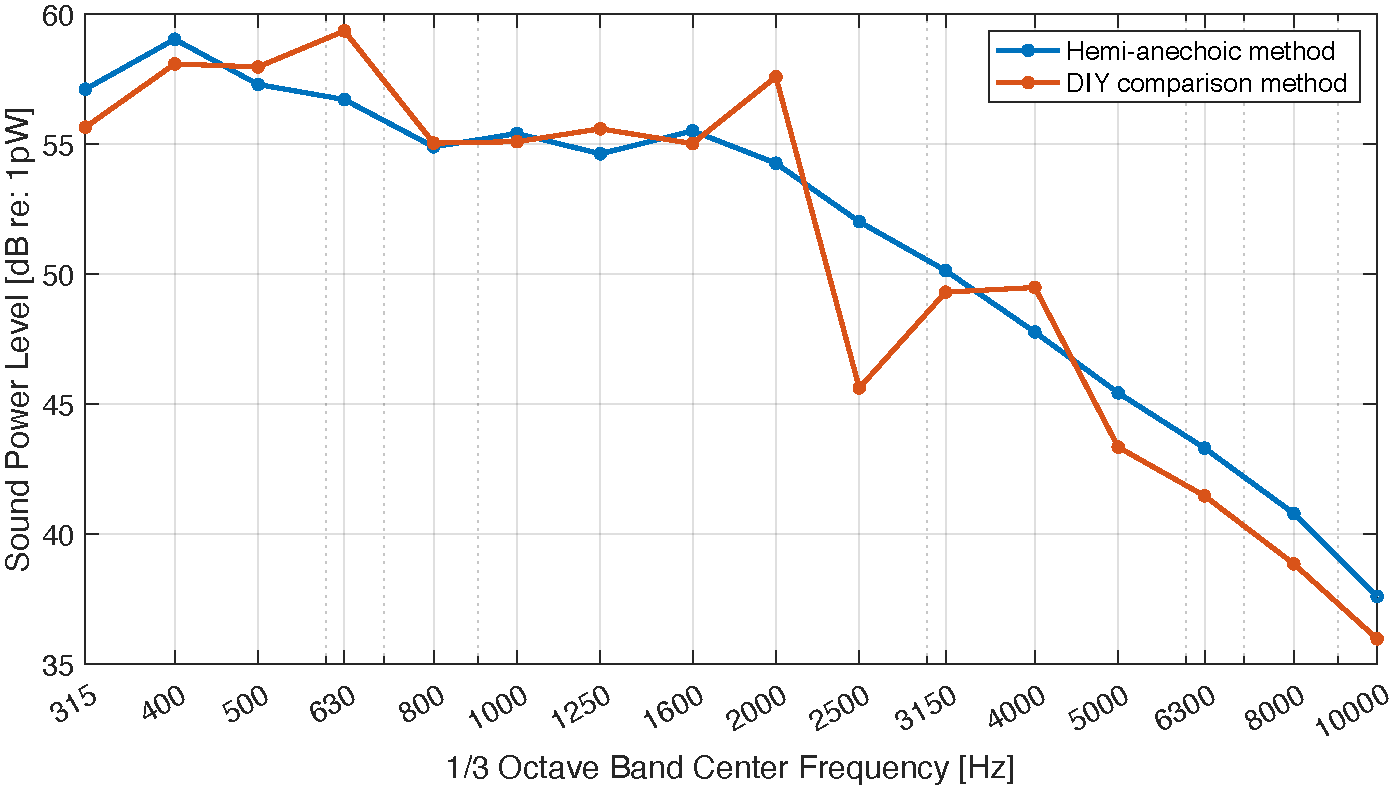
\includegraphics[width=0.9\textwidth]{manuscript/fig/VacComparison.pdf}
          \caption{Sound power level of the Corsi-Rosenthal Box at fan setting 3 as measured with the hemi-anechoic method and the DIY comparison method.}
        \label{fig:comparisonfan3}
\end{figure}

\clearpage
\section{Discussion and Conclusions}
The results presented here provide a groundwork for future investigations into DIY sound power measurements. Several common everyday objects were thought to be promising candidates for an inexpensive, repeatable broadband sound power source.  Small hand vacuums had the best overall attributes from our pool of chosen objects. When the hand vacuums were used as a reference source, they showed a promising similarity to the ``ground truth'' sound power measured using the hemi-anechoic method.

To allow for more accessible measurements, a smartphone based SLM application could be used.  Kardous and Shaw have done several studies evaluating many different smartphones and applications on their viability for use as SLMs \cite{kardous2014evaluation, kardous2015sound, kardous2016evaluation}. They found that iPhone applications \textit{NoiSee}, \textit{SoundMeter} and \textit{SPLnFFT} all met the $\pm2$ dB criteria for unweighted measurements and that \textit{NoiseHunter}, \textit{NoiSee} and \textit{SoundMeter} all had mean differences within $\pm2$ dBA for the weighted measurements. All of the Android applications tested had a high variance of measurement and lacked feature and manufacturing conformity between devices.

This study was limited by several factors. First, the facility used for the hemi-anechoic method was not large enough to fulfill the size requirements of the standard. In addition, frequencies below 300 Hz could not accurately be measured due to room dimensions and construction. Second, the small sample size of tested objects did not fully canvas what was available on the market. Other options may provide more favorable results. Last, only one environment was tested in the comparison method as a proof of concept. Multiple environments could be used to validate the comparison results.

Future work might include testing in additional environments, exploring different reference sources and increasing the hand vacuum sample size along with multiple Corsi-Rosenthal boxes. 

\noindent

\section*{Acknowledgments}
\noindent
We would like to thank the Penn State Graduate Program in Acoustics for funding this work. We would also like to thank Olivia Park and Zane Rusk of SPRAL at Penn State for letting us use their anechoic facility. Lastly, we would like to thank the team that inspired this work: David Elfstrom, Rob Wissmann and Stefan Stojanovic.
\bibliographystyle{unsrt}
\bibliography{refs} 

\end{document}

